\section{Introduction}


Large Language Models (LLMs) have rapidly evolved from simple chatbots into capable systems that can write code, control browsers, and perform advanced question answering~\citep{comanici2025gemini}. These advances have been driven by improving inference, planning, and tool use, as shown by benchmarks emphasizing logical reasoning and multi-step actions. Yet a fundamental capability, \emph{memory}, remains largely underexplored. Memory allows LLMs to maintain state across interactions, accumulate experience, and adapt strategies over time. Recent studies have introduced memory modules that track dialogue histories through compression, indexing, or retrieval~\citep{maharana2024evaluating}, improving \emph{conversational recall} and personalization. However, most of these systems only reuse static dialogue context rather than learning from experience to improve future reasoning or decision-making.






Despite these advances, existing LLM memory systems remain largely static, retrieving information passively rather than evolving through use. Current evaluations test whether models can recall past context but rarely assess their ability to \emph{reuse experience}. In essence, agents remember what was said but not what was learned. \emph{Conversational recall} retrieves prior facts, whereas \emph{experience reuse} abstracts reasoning strategies for future tasks. Without such reuse, models repeatedly solve similar problems, as long-term assistants often recall context yet fail to adapt across sessions. 

\begin{wrapfigure}{r}{0.55\textwidth}
    \centering
    % \vspace{-10pt} % 控制图与上文的间距
    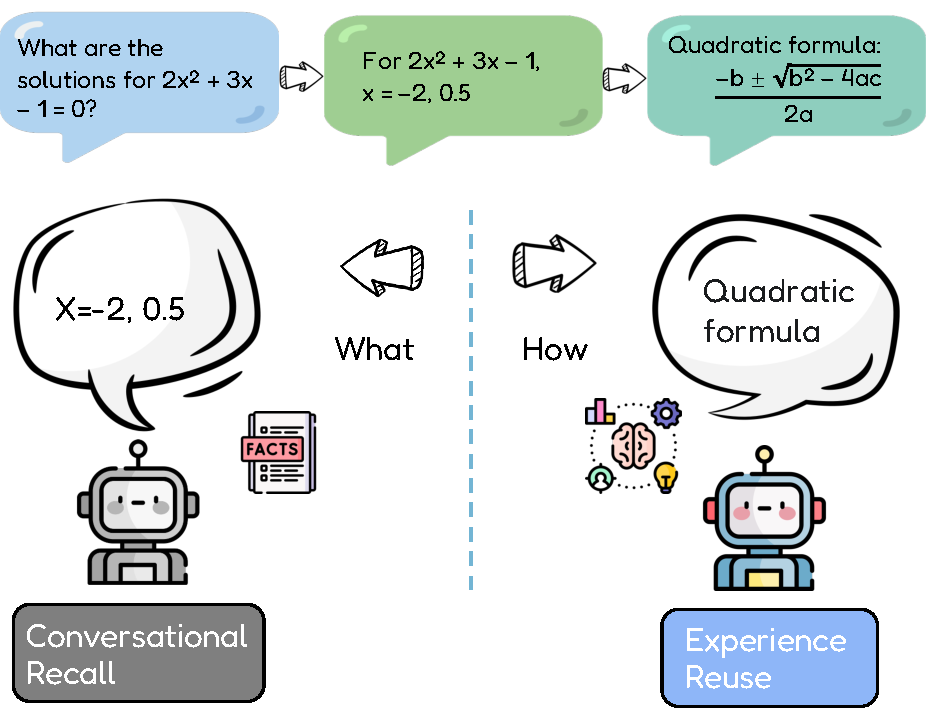
\includegraphics[width=\linewidth]{figures/compare_figure.pdf}
    \caption{Conversational recall retrieves past facts (e.g., solutions to $2x^2 + 3x - 1 = 0$).
Experience reuse recalls reasoning strategies (e.g., using the formula).}
    \label{fig:compare}
    % \vspace{-10pt} % 控制图与下文的间距
\end{wrapfigure}

Several recent benchmarks have begun examining static adaptation but remain limited in scope. StreamBench~\citep{wu2024streambench} evaluates sequential learning but mainly measures factual retention without reasoning or trajectory reuse. LifelongBench~\citep{zheng2025lifelongagentbench} studies lifelong learning across environments and skills but focuses on retention without modeling memory structure or updates. Other studies~\citep{hu2025evaluating,wulongmemeval,maharana2024evaluating} assess long-term conversational consistency but do not test how agents evolve their memory during deployment. Together, these efforts highlight a critical gap: while progress has been made on sequential reasoning, there is still no unified framework for evaluating how different memory methods retrieve, integrate, and evolve historical strategies in realistic streaming scenarios. Figure~\ref{fig:compare} illustrates this contrast between static recall and cumulative improvement through self-evolving memory. 




\begin{figure}[t]
    \centering
    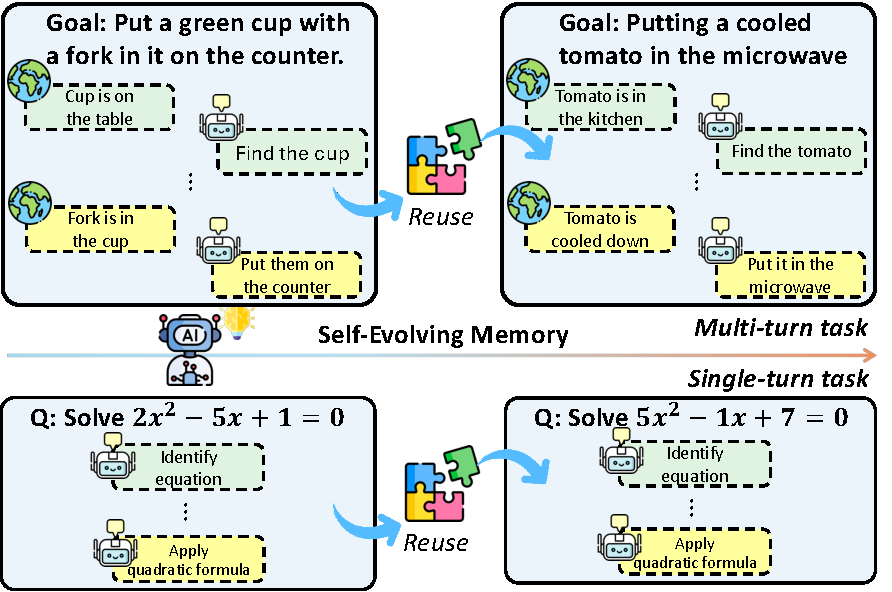
\includegraphics[width=0.8\linewidth]{figures/teaser.pdf}
    \caption{Illustration of different task types and experience reusing. A stateful agent encounters both multi-turn tasks (e.g., embodied manipulation) and single-turn tasks (e.g., solving equations), and should learn reusable experiences from past experiences.}
    \label{fig:compare_task}
\end{figure}



To bridge this gap, we introduce \textbf{\method}, a comprehensive streaming benchmark and framework for evaluating \emph{self-evolving memory} in LLM agents. Figure~\ref{fig:compare_task} illustrates how a self-evolving agent reuses prior experiences across both multi-turn interactive tasks and single-turn reasoning tasks. \method restructures datasets into sequential \emph{task streams}, requiring models to retrieve, adapt, and evolve memory after each interaction. The benchmark covers both \emph{multi-turn goal-oriented} environments and \emph{single-turn reasoning or problem-solving} tasks, explicitly testing whether LLMs can accumulate knowledge and refine strategies during deployment, a process we term \emph{test-time evolution}. We unify and implement over ten representative memory modules, including retrieval-based, workflow, and hierarchical memory systems, to study their adaptation behavior. To further examine experience reuse, we introduce \textbf{ExpRAG}, a simple retrieval-based baseline that leverages prior task experiences, and further develop \textbf{\alg}, an advanced \emph{action–think–memory refine} pipeline that tightly integrates reasoning, action, and memory updates for continual improvement.

In summary, our contributions are threefold:
\begin{itemize}[itemsep=0pt,topsep=2pt,leftmargin=*]
    \item \textbf{Benchmark:} We present \method, a streaming benchmark that evaluates LLM agents' ability to perform \emph{test-time evolution} across diverse multi-turn and single-turn tasks, bridging the gap between conversational recall and experience reuse.
    \item \textbf{Framework:} We provide a unified evaluation framework with memory-centric metrics for analyzing adaptation, efficiency, and stability, and will release all code and configurations for reproducibility.
\item \textbf{Analysis and Insights:} We introduce \textbf{ExpRAG}, a simple retrieval-based baseline for experience reuse, and \textbf{\alg}, an \emph{action–think–memory refine} pipeline that unifies reasoning, action, and memory for continual improvement, informing future designs of memory.
\end{itemize}



